\subsubsection{Descrizione generale}
La classe \verb+SorterService+ si occupa del servizio di sorting di uno o più post: innanzitutto fornisce l'entry point per sfruttare il servizio Amazon AWS Rekognition, dopo di che sono implementate tutte le funzioni contenenti l'effettiva algoritmica di sorting per il calcolo del punteggio del post dalle sue immagini.

Più nello specifico, \verb+SorterService+ implementa:
\begin{lstlisting}[language=Python]
    def __init__(self):
    self._rekognition = boto3.client(
    service_name='rekognition', region_name=aws_region
    )
\end{lstlisting} 
che si occupa di fornire un handle sotto forma di oggetto per accedere al servizio AWS Rekognition
(\verb+self._rekognition+). 
Poi definisce e implementa le seguenti funzioni:
\begin{itemize}
	\item 
	\begin{lstlisting}[language=Python, numbers=none]
def process_event(self, event: SortEvent) -> dict:
	\end{lstlisting}
Entry point per la funzione di sorting; si occupa di lanciare il servizio di sorting sui post salvati. Ritorna infine una lista con tutti i post validi;
	\item 
	\begin{lstlisting}[language=Python, numbers=none]
def sort(self, post: SortingPost) -> Optional[SortingPost]:
	\end{lstlisting}
Chiama una funzione per calcolare lo score di un post dalle sue immagini. Se è possibile calcolare lo score di un post esso viene ritornato a \verb+process_event+; Se invece non è possibile viene evocato la funzione \verb+_delete_post+ a cui viene passato il post da eliminare;
	\item 
	\begin{lstlisting}[language=Python, numbers=none]
def _delete_post(self, post: SortingPost):
	\end{lstlisting}		
Si occupa di eliminare il post inutilizzabile e di rimuovere le sua immagini dal bucket di S3 su cui erano state salvate;
	\item 
	\begin{lstlisting}[language=Python, numbers=none]
def calculate_image_score(self, post: SortingPost):
	\end{lstlisting}	
Si occupa inizialmente di calcolare lo score di ogni singola immagine di un post e dopo di che calcola lo score finale dell'insieme di immagini del post;
	\item
	\begin{lstlisting}[language=Python, numbers=none]
def analyze_image(self, name_image: str):
	\end{lstlisting}	
Verifica che siano presenti persone nella foto(\verb+detect_person+) ed emozioni(\verb+detect_sentiment_person+). Ritorna, se presenti, un dizionario di emozioni e un dizionario dei rispettivi valori numerici;
	\item 
	\begin{lstlisting}[language=Python, numbers=none]
def detect_sentiment_person(self, name_image: str):
	\end{lstlisting}	
Utilizza il servizio AWS Rekognition per riconoscere le facce ed emozioni correlate in un immagine. Controllerà che le emozioni siano valide(devono avere un valore pari o superiore al 90\% per essere considerate influenti sullo score finale) e verrà poi creato e ritornato a \verb+analyze_image+ un dizionario dei sentimenti, un dizionario dei rispettivi valori numerici e un booleano per segnalare di aver trovato o meno emozioni;
	\item
	\begin{lstlisting}[language=Python, numbers=none]	
def detect_person(self, name_image: str):
	\end{lstlisting}	
Utilizza il servizio di AWS Rekognition per analizzare l'immagine e riconoscere delle labels; queste labels verranno controllate per verificare la presenza di persone. Verrà ritornato un booleano per segnalare la presenza o meno di persone.
\end{itemize}
\newpage
\subsubsection{Diagramma delle classi}
\begin{figure}[!h]
    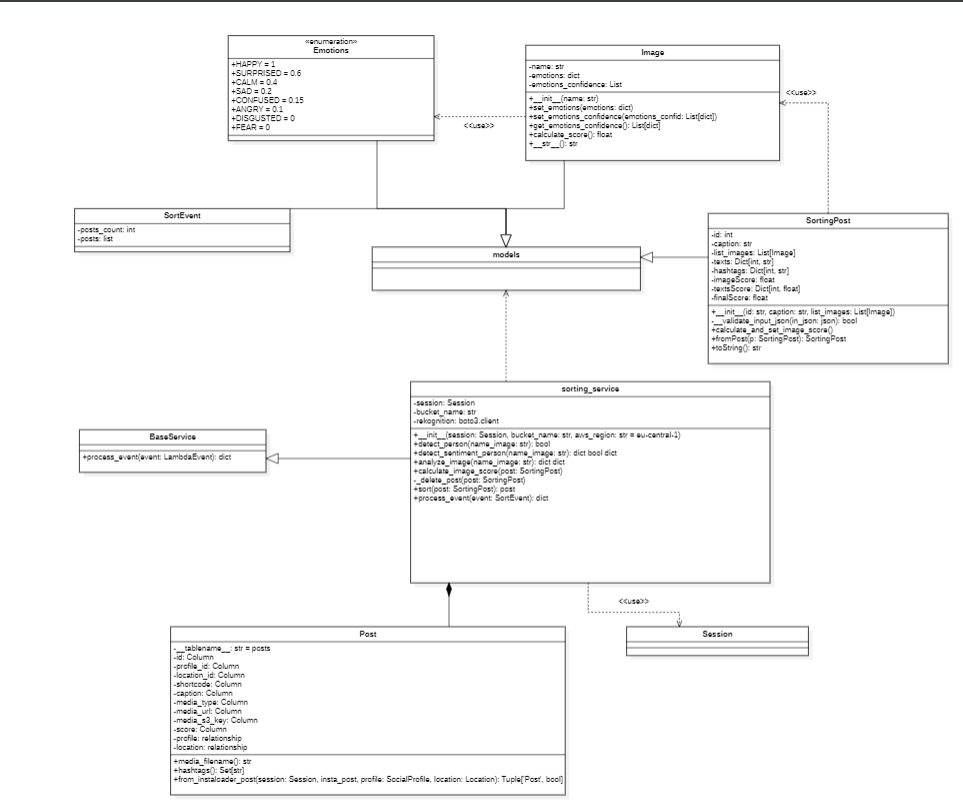
\includegraphics[width=15cm]{sezioni/images/cd_sorting.png}
    \caption{Sorting Service - Diagramma delle classi}
\end{figure}
\subsubsection{Diagrammi di sequenza}

\subsubsection{Schemi I/O}
\paragraph*{Input} esempio di evento in input, in formato JSON\G{}.
\begin{lstlisting}[language=JSON]
{
    "posts_count": 4,
    "posts": [
        {"id": 1},
        {"id": 2},
        {"id": 3},
        {"id": 4}
    ]
}
\end{lstlisting}
Descrizione:
\begin{itemize}
    \item \verb|posts_count|: numero di post di cui effettuare il sorting;
    \item \verb|posts|: array di post. 
\end{itemize}

\paragraph*{Output} esempio di risposta in output, in formato JSON\G{}.
\begin{lstlisting}[language=JSON]
{
    "posts_count": 2,
    "posts": [
        {"id": 2},
        {"id": 4}
    ]
}
\end{lstlisting}
Descrizione:
\begin{itemize}
    \item \verb|posts_count|: numero di post tenuto dopo il sorting;
    \item \verb|posts|: array di post. 
\end{itemize}

\subsubsection{Calcolo dell'imageScore}
Segue una spiegazione più dettagliata del processo per il calcolo di imageScore necessario al sort dei post.
\paragraph{Inizio processo} \aCapo{}
Il processo inizia con \verb+process_event(self, event: SortEvent) -> dict+ che si occupa di prendere dal database i post sui quali chiamerà la funzione \verb+sort+.
\begin{lstlisting}[language=Python]
        for p in event.posts:
        db_post = self._session.query(models.Post).filter_by(id=p['id']).first()
        sorting_post = SortingPost.fromPost(db_post)
        sorting_post = self.sort(sorting_post)
\end{lstlisting} 
Essa chiamerà a sua volta \verb+calculate_image_score+ che con un dizionario di emozioni e un dizionario sulla confidenza di tali emozioni permette il calcolo di imageScore.
\begin{lstlisting}[language=Python]
        self.calculate_image_score(post)
\end{lstlisting}
\begin{lstlisting}[language=Python]
        image.set_emotions(emotions)
        image.set_emotions_confidence(emotions_confidence)

        post.calculate_and_set_image_score())
\end{lstlisting} 
\paragraph{Creazione e uso dei dizionari} \aCapo{}
Per creare tale dizionari si utilizza la funzione \verb+detect_sentiment_person+ che utilizzerà a sua volta il servizio AWS Rekognition per il riconoscimento delle facce ed eseguirà poi un analisi sulla risposta ritornata dal servizio. Attraverso tale analisi si salveranno solo le emozioni valide ossia con una confidenza pari o superiore al 90\%. Verranno ritornati i dizionari a \verb+calculate_image_score+ dove verranno usati per salvare le emozioni valide nell'oggetto "Image" nel seguente modo:
\begin{lstlisting}[language=Python]
    def set_emotions(self, emotions: dict):
        self.emotions = emotions

    def set_emotions_confidence(self, emotions_confid: List[dict]):
        self.emotions_confidence = emotions_confid
\end{lstlisting}
\paragraph{Calcolo finale} \aCapo{}
Il calcolo finale di imageScore avviene con il seguente algoritmo chiamato \verb+calculate_and_set_image_score+: 
\begin{lstlisting}[language=Python]
        if self.list_images:
            count = 0
            for image in self.list_images:
                score = image.calculate_score()
                if score is not None:
                    count += 1
                    self.imageScore = (
                        (self.imageScore + score)
                        if self.imageScore is not None
                        else score
                    )
            if self.imageScore:
                self.imageScore = self.imageScore / count
\end{lstlisting}
dove lo score delle singole immagini viene calcolato con l'algoritmo chiamato \verb+calculate_score+:
\begin{lstlisting}[language=Python]
        if self.emotions:
            value_sum = 0.0
            sum_weights = 0.0
            for emotion, num in self.emotions.items():
                value_sum += Emotions[emotion].value * num
                sum_weights += num
            return 100 * value_sum / sum_weights
        else:
            return None
\end{lstlisting}
\paragraph{Conclusione processo} \aCapo{}
Se l'imageScore sarà stato calcolato il post è valido e verrà tenuto; se invece non è stato calcolato significa che il post non è valido e sarà eliminato insieme alle sua immagini salvate su un bucket S3 tramite la funzione \verb+_delete_post+:
\begin{lstlisting}[language=Python]
        for img in post.list_images:
            s3_delete_file(self._bucket_name, img.name)
        self._session.delete(
            self._session.query(models.Post).filter_by(id=post.id).first()
        )
        self._session.commit()
\end{lstlisting}
\subsubsection{Variabili}
Segue una spiegazione più dettagliata di alcune variabili usate dagli algoritmi spiegati precedentemente:
\paragraph{Response from detect\textunderscore{}faces} \aCapo{}
	\begin{lstlisting}[language=Python]
response = self._rekognition.detect_faces(
            Image={'S3Object': {'Bucket': self._bucket_name, 'Name': name_image}},
            Attributes=['ALL'],
        )
	\end{lstlisting}
	La variabile response riceve il risultato della funzione \verb+detect_faces+ del servizio AWS Rekognition; tale funzione prende in input un'immagine presente in un bucket di S3 e ritorna come risultato un file JSON\G{} contente  una sentiment analysis dei volti presenti nell'immagine. Segue un esempio ove presenti solo i dati necessari al nostro caso:
	\begin{lstlisting}[language=JSON]
    {
    "FaceDetails": [
        {
        	....
        	....
            "Emotions": [
                {
                    "Type": "ANGRY",
                    "Confidence": 55.18563461303711
                },
                {
                    "Type": "HAPPY",
                    "Confidence": 37.01131820678711
                },{},{},{},{},{},{}
            ],
            ....
            ....
            ....
            ....
        }
    }
	\end{lstlisting}
	Tale risultato sarà usato dalla funzione \verb+detect_sentiment_person+ per creare  un dizionario di emozioni e
un dizionario sulla confidenza di tali emozioni nel seguente modo:
	\begin{lstlisting}[language=Python]
		contain_emotion = False
        emotions_dict = {}
        emotions_confid = []

        for faceDetail in response['FaceDetails']:
            emotions = faceDetail['Emotions']
            confid_single_face = {}
            for emotion in emotions:
                emotion_name = emotion['Type']
                emotion_confid_value = emotion['Confidence']
                if emotion_name != 'UNKNOWN':
                    confid_single_face[emotion_name] = emotion_confid_value

                    if emotion_confid_value >= 90:
                        if emotion_name in emotions_dict:
                            emotions_dict[emotion_name] += 1
                        else:
                            emotions_dict[emotion_name] = 1
                        contain_emotion = True
            emotions_confid.append(confid_single_face)
        return emotions_dict, contain_emotion, emotions_confid
	\end{lstlisting}
\paragraph{Response from detect\textunderscore{}labels} \aCapo{}
	\begin{lstlisting}[language=Python]
response = self._rekognition.detect_labels(
            Image={'S3Object': {'Bucket': self._bucket_name, 'Name': name_image}},
            MaxLabels=10,
        )
	\end{lstlisting}
La variabile response riceve il risultato della funzione \verb+detect_labels+ del servizio AWS Rekognition; tale funzione prende in input un'immagine presente in un bucket di S3 e ritorna come risultato un file JSON\G{} contente una labels analysis delle istanze di entità del mondo reale presenti nell'immagine. Segue un esempio ove presenti solo i dati necessari al nostro caso:
\begin{lstlisting}[language=JSON]
	{
		"Labels": [

			{
				"Name": "Person",
                "Confidence": 99.88428497314453,
                "Instances": [
                	{
                    	"BoundingBox": {
                        "Width": 0.27858132123947144,
                        "Height": 0.44550982117652893,
                        "Left": 0.2236727923154831,
                        "Top": 0.35303789377212524
                         },
                     "Confidence": 99.88428497314453
                    },
					{
                        "BoundingBox": {
                        "Width": 0.20297367870807648,
                        "Height": 0.6778767108917236,
                        "Left": 0.5247262716293335,
                        "Top": 0.10922279208898544
                      	 },
                    "Confidence": 99.81658172607422
					}
				]
                ....
                ....
                ....
                ....
            	....
		}]
	}
	\end{lstlisting}
Tale risultato sarà usato dalla funzione \verb+detect_person+ per verificare la presenza di persone nel seguente modo:
\begin{lstlisting}[language=Python]
		contain_person = False

        for label in response['Labels']:
            if label['Confidence'] >= 90:
                if label['Name'] == 'Person':
                    contain_person = True

        return contain_person
\end{lstlisting}
In questo nostro esempio possiamo vedere, nel file JSON\G{}, che sono presenti due persone indicate dal parametro "BoundingBox". La funzione sopra vedrà la presenza di queste due persone e tornerà un risultato positivo alla funzione \verb+analyze_image+ che quindi saprà di poter chiamare la funzione \verb+detect_sentiment_person+ il cui scopo è descritto sopra.
